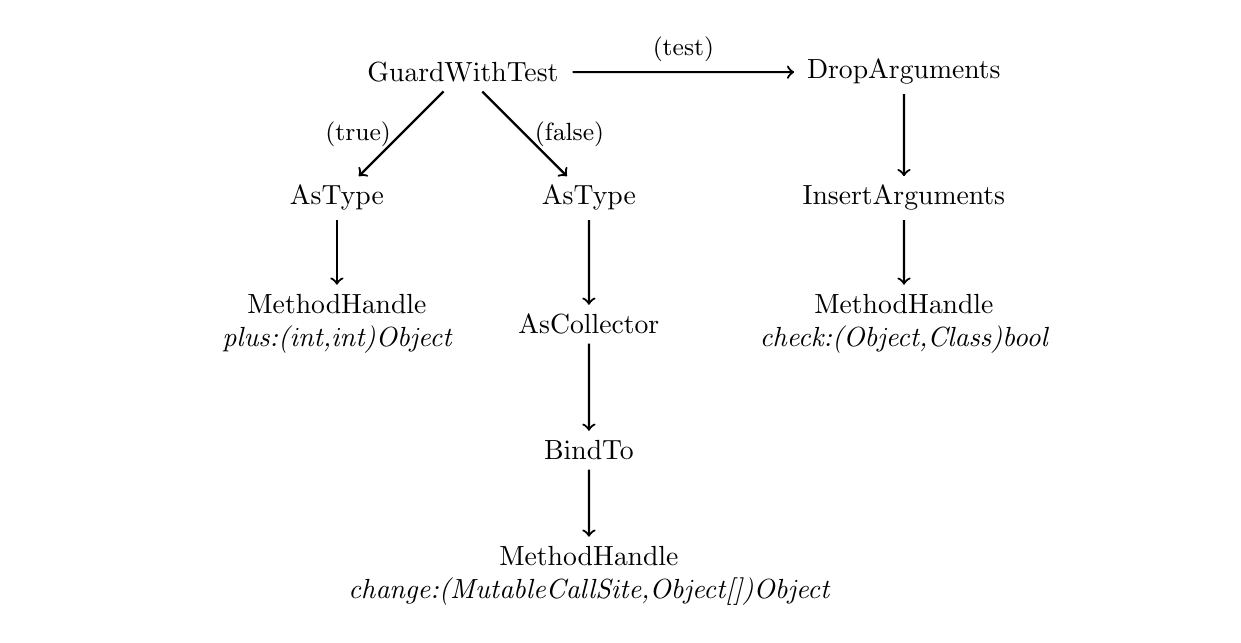
\begin{tikzpicture}[scale=1.6]
  \node[text width=3in,align=center](A1) at (2,-2){AsType};
  \node[text width=3in,align=center](A2) at (2,-3){AsCollector};
  \node[text width=3in,align=center](A3) at (2,-4){BindTo};
  \node[text width=3in,align=center](A4) at (2,-5){MethodHandle\\{\it change:(MutableCallSite,Object[])Object}};

  \node[text width=1in,align=center](G1) at (1,-1){GuardWithTest};

  \node[text width=3in,align=center](B1) at (0,-2){AsType};
  \node[text width=3in,align=center](B2) at (0,-3){MethodHandle\\{\it plus:(int,int)Object}};

  \node[text width=1in,align=center](C1) at (4.5,-1){DropArguments};
  \node[text width=3in,align=center](C2) at (4.5,-2){InsertArguments};
  \node[text width=3in,align=center](C3) at (4.5,-3){MethodHandle\\{\it check:(Object,Class)bool}};

  \draw[thick,->](A1) -- (A2);
  \draw[thick,->](A2) -- (A3);
  \draw[thick,->](A3) -- (A4);
  \draw[thick,->](B1) -- (B2);

  \draw[thick,->](C1) -- (C2);
  \draw[thick,->](C2) -- (C3);
  \draw[thick,->](G1) -- node[right] {\small (false)} (A1);
  \draw[thick,->](G1) -- node[left]  {\small (true)}  (B1);
  \draw[thick,->](G1) -- node[above] {\small (test)}  (C1);
\end{tikzpicture}
